\section{Bias and Variance for Learning in 1-D}
In this project, you will compare the difference between \textit{approximation} (finding the best possible candidate to model a function) and \textit{learning} (finding the best possible candidate given limited information). You will analyze the extra error incurred by using limited information, and explore one possible way of reducing this error.\\

\noindent\textit{Approximation:}\\
Let $f(x) = x^2(1-x)$ where $0 \leq x \leq 1$. We wish to find the `best' linear model (or approximation) for $f$. That is, for functions in the form $g(x; \alpha, \beta) =  \alpha +  \beta x$,  we wish to find the parameters $ \alpha$ and $ \beta$ that minimize the error we would expect to incur if we used the function $g$ to model (or approximate) the function $f$. 
\begin{center}
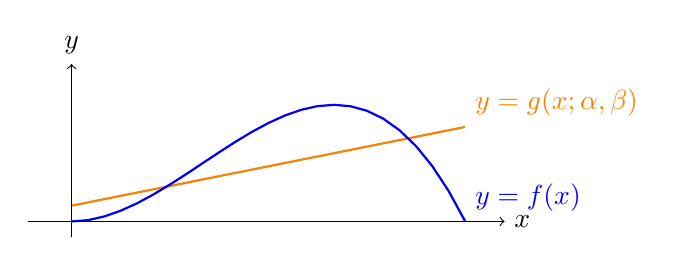
\begin{tikzpicture}[xscale=5,yscale=10]
% \draw[densely dotted] (-.2,-.2) grid (1.2,0.3);
\draw[thick,domain=0:1,variable=\x,orange] plot ({\x},{.02 + .1*\x}) node[above right] {$y = g(x; \alpha, \beta)$};
\draw[thick,domain=0:1,variable=\x,blue] plot ({\x},{\x*\x*(1-\x)}) node[above right] {$y = f(x)$};
  \draw[->] (-.11, 0) -- (1.1, 0) node[right] {$x$};
  \draw[->] (0, -.02) -- (0, .2) node[above] {$y$};
\end{tikzpicture}
\end{center}
For this problem, we will define the error as
\begin{equation*}
\text{Error}(x;\alpha,\beta) = \bigg(f(x) - g(x; \alpha, \beta)\bigg)^2 
\quad \text{and} \quad
\text{TotalError}(\alpha,\beta) = \int_0^1 \text{Error}(x; \alpha,\beta) dx.
% \text{Error}(f,g) = \int_0^1 \bigg(f(x) - g(x; \alpha, \beta)\bigg)^2 dx.
\end{equation*} 
Use pencil-and-paper (or Mathematica, WolframAlpha, etc) to find a simplified expression for the error between $f$ and $g$ as a function of the parameters $ \alpha$ and $ \beta$. Find the values of $ \alpha$ and $ \beta$ that minimize the total error and find the corresponding total error.\\

\noindent\textit{Learning:}\\
In many practical applications, we only have imperfect knowledge of $f$, and therefore it is impossible to know the \textit{best possible} parameters $\alpha, \beta$. 
Often, we must commit to a choice of sub-optimal parameters that are chosen after only a small glimpse of $f$. 
In this project, you will estimate and explore the extra error incurred when using an imperfect choice of parameters.\\
\noindent\textit{Terminology:} Bias\\
\noindent\textit{Terminology:} Variance.\\
Implement the following process to estimate how well a linear function parameterized by two random data points can be used to model $f$.\\

\noindent Create the variable \texttt{xx} by discretizing the $x$ interval $0 \leq x \leq 1$ into 101 points. 
That is, set \texttt{xx}$ = (0,\, 0.01,\, 0.02,\, \dots,\, 1)$.

\noindent Loop until you are confident you have reasonably accurate answers.
\begin{enumerate}\setlength{\itemsep}{0pt}
    \item Generate two random data points on $x_1, x_2 \in [0,1]$.
    \item Evaluate $y_1 =f(x_1)$ and $y_2 = f(x_2)$.
    \item Using \textbf{only} $(x_1,y_1)$ and $(x_2,y_2)$, compute a `best guess' for parameters $\alpha$ and $\beta$.
    \item Use your best guess parameters $\alpha$ and $\beta$ to evaluate the linear model $g(x;\alpha, \beta)$ for each $x \in \texttt{xx}$. Record the results.
\end{enumerate}
Plot the $\bar{g}(x)$, the average prediction given by the linear model for each $x$. 
On the same figure, plot $g_{5}(x)$, $g_{25}(x)$, $g_{75}(x)$ and $g_{95}(x)$, the 5\textsuperscript{th}, 25\textsuperscript{th}, 75\textsuperscript{th} and 95\textsuperscript{th} quantiles of the prediction values given by the linear model.  
Compute the bias and the variance of the linear model when it is trained on two data points. \\

\noindent\textit{Error reduction for Learning:}\\
Someone proposes that the variance is so big that it makes the linear model unusable.  
They suggest that we should approximate $f$ by a constant function  $h(x;\alpha)$. 
Repeat the steps above to compute the bias and to the estimate the variance of the constant model. \\


